\def\chapterabstract{In this chapter, we present a set of methods designed for tracking with high-order accuracy the propagation of surfaces in three dimensions with arbitrary geometric and topological complexity. Targeted applications are engineering and scientific problems for which a CAD (computer-aided design) model of the geometry is available, i.e. surface patches with high-order parameterizations as well as topological connectivity. Our method uses and maintains such a representation throughout the propagation. Validity of the dynamic boundary-representation model is ensured by handling geometric singularities. Examples are presented to demonstrate the accuracy of the pseudo-spectral method used for tracking each surface patch.
A strategy for deriving a dynamic surface mesh is finally proposed for applications such as Finite Element/Volume computations with body-fitted volume grids in domains with deforming boundaries. }

%\chapter{A chapter with short title}
%\chapter{Développement d'une méthode pseudo-spectrale pour le suivi d'un patch rectangulaire de surface}
%\chapter{Méthode pseudo-spectrale pour le suivi d'un patch rectangulaire de surface}
\chapter{Déformation de maillage surfacique}
%\epigraph{ Some fancy epigraph. }{ Anonym }

%\begin{abstract}
\printskip
\printchapapp
The work presented in this chapter focuses on surface propagation problems in industrial or scientific applications for which a CAD model of the geometry is available. The method presented in the following section takes this particular definition as a starting point and extends it to evolving geometries. \par
%\end{abstract}

Some \textbf{bold} text. Some \textit{italics} text. Some \emph{emphasized} text. Some \textsf{sans serif} text. Some \texttt{typewriter} text. {\color{myred} Some text in \textbf{red} \ldots} {\color{mygreen} Some text in \textbf{green} \ldots} \par
Mathcal $\mathcal{ABCDEFGHIJKLMNOPQRSTUVWXYZ}$.\\
Numbers: 1234567890, in math mode: $1234567890$.\\
{\scshape Small caps, in \textbf{bold}, in \textit{italics}.}

\newlength\TestLength
\setlength{\TestLength}{0pt}
\begin{figure}[htp]
  \centering
  \begin{tikzpicture}
    \node[rectangle,draw=red] (n) at (4,3) {abc};
    \getwidthofnode{\TestLength}{n}
    \node[anchor=north east] at (n.south west) {width = \the\TestLength};
    \getheightofnode{\TestLength}{n}
    \node[anchor=north west] at (n.south east) {height = \the\TestLength};
  \end{tikzpicture}
\end{figure}
TestLength = \the\TestLength.

\section{A section}

\paragraph*{Definition}
The $n$-th Chebyshev polynomial (of the first kind) $T_n$ is a polynomial of degree $n$ defined by
\begin{equation*}
	T_n \left(\cos \theta \right) = \cos n \theta.
    \label{def_cos}
\end{equation*}

For $x \in \chebinterval$, $T_0(x) = 1$, $T_1(x) = x$ and from the trigonometric identity $\cos n\theta + \cos (n-2)\theta = 2\cos \theta \cos (n-1)\theta $ the following recurrence relation can be derived
\begin{equation}
	T_{n}(x) = 2x T_{n-1}(x) - T_{n-2}(x) \quad, \quad n \geq 2.
    \label{eq:recurrence}
\end{equation}
Relation (\ref{eq:recurrence}) allows efficient evaluation of Chebyshev polynomials, e.g. via Clenshaw's algorithm \cite{clenshaw1955}. %The first five \cheb polynomials are plotted on {\modif Fig.} \ref{fig:poly_cheb}.
\par

On the interval $\chebinterval$, $T_n$ reaches its extremal values at the $n+1$ \textit{Chebyshev-Gauss-Lobatto} (CGL) points
\begin{equation*}
	\hat{x}_k = \cos \frac{k \pi}{n} \quad, \quad k = 0,\ldots,n.
\end{equation*}
\subsection{A subsection}

\begin{equation}
	\boldsymbol{f}(u,v) = \sum_{m = 0}^\infty \sum_{n = 0}^\infty \boldsymbol{c}_{mn} T_m(u) T_n(v) .
\end{equation}
Math macros\footnote{This is a footnote.} are tested in \Cref{sec:testmathmacros}.
\lipsum


\Cref{eq:recurrence} is an equation, \Cref{def_cos} is an equation, \Cref{fig0} is a figure. \fref{fig0} is a figure.

\begin{figure}
\centering
%\includegraphics[height=45mm]{/d/bandrieu/stck/Bureau/Figures/Degenerate/im_00}
\caption{Lagrangian transport may lead to mesh degeneracy.}
\label{fig0}
\end{figure}


\section{Another section}
\paragraph{Paragraph.}

\begin{figure}
	\centering
	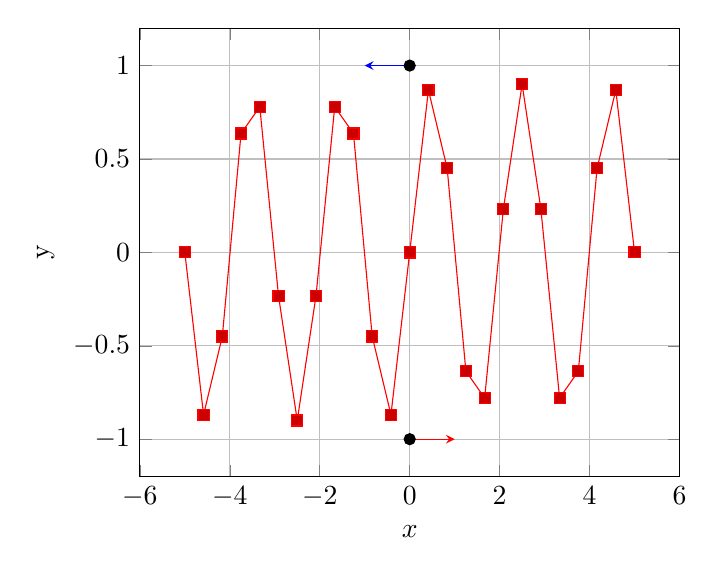
\begin{tikzpicture} 
		\begin{axis}[grid=major, xlabel=$x$, ylabel=y]
			\draw[red,-stealth] (axis cs:0,-1) 
				-- % = line-to 
				++ % = calculate a vector sum 
				(axis direction cs:1,0); 
			\addplot [only marks,mark=*] 
				coordinates { (0,-1) (0,1) }; 
			\draw[blue,-stealth] (axis cs:0,1) 
				--
				++ 
				(axis direction cs:-1,0); 
			\addplot {0.9*sin(180*x)};
%			\addlegendimage{empty legend}
%			\addlegendentry[text width=9em,text depth=]%
%			{The quick brown fox jumps over the lazy dog.}
		\end{axis} 
	\end{tikzpicture}
	\caption{Test pfgplot}
\end{figure}

\begin{figure}
	\centering
	\begin{tikzpicture} 
		\begin{loglogaxis}[%
			width=8cm, height=6cm,%
			xmin=1.0e2, xmax=1.0e4, ymin=1.0e-15, ymax=1.0,%
			grid=both,%
			xlabel={nombre total de marqueurs surfaciques},%
			ylabel={Erreur},%
			legend pos=south west,%
			legend style={font=\small},%
			]%
			\addplot+ table[x index=0, y index=1] {figures/data/test.dat}; 
			\addplot+ table[x index=0, y index=2] {figures/data/test.dat}; 
			\addplot+ table[x index=0, y index=3] {figures/data/test.dat}; 
%			\addplot+ coordinates {
%				(2e2, 1e-2) (6e2, 1e-3) (2e3, 1e-7) (6e3, 1e-12)
%				};
%			\addplot+[smooth] coordinates {
%				(1e3, 1e-14) (2e3, 1e-6) (4e3, 1e-2) (6e3, 1e-11) (8e3, 1e-13)
%				};
%			\addplot+[smooth] coordinates {
%				(1e3, 1e-1) (2e3, 1e-9) (4e3, 1e-13) (6e3, 1e-4) (8e3, 1e-2)
%				};	
%			\addplot+[smooth, dashed, no marks] coordinates {
%				(1.3e2, 1e-2) (5e2, 1e-4) (2e3, 1e-9) (4e3, 1e-13) (7e3, 1e-14)
%				};
%			\addplot+[smooth, dotted, no marks] coordinates {
%				(1.3e2, 1e-13) (5e2, 1e-11) (2e3, 1e-6) (4e3, 1e-2) (7e3, 1e-1)
%				};
			\legend{{position}, {aire}, {volume}, {toto}, {riri}, {fifi}, {loulou}, {babar}} 
		\end{loglogaxis} 
	\end{tikzpicture}
	\caption{Test pfgplot loglog}
\end{figure}

\begin{figure}
	\centering
	\begin{tikzpicture} 
		\begin{axis}[%
			width=8cm, height=6cm,%
		 	% load a color `cycle list' from the `colorbrewer' library
			cycle list/Spectral-6,%RdYlBu-6,%
            % create new `cycle list` from existing `cycle list's and an
            cycle multiindex* list={
                set1%Spectral-6%RdYlBu-6%
                    \nextlist%
                no marks%
                	\nextlist%
                thick
            },%
			xmin=-1.0, xmax=1.0, ymin=-1.0, ymax=1.0,%
			grid=major,%
			enlargelimits={abs=0.05},
			xlabel={$x$},%
			ylabel={$T_n(x)$},%
			legend style={at={(1.025,0.5)}, anchor=west},%
			samples=200%
			]%
			\addplot+[domain=-1:1] {1.0};
			\addplot+[domain=-1:1] {x};
			\addplot+[domain=-1:1] {2.0*x^2 - 1.0};
			\addplot+[domain=-1:1] {4.0*x^3 - 3.0*x};
			\addplot+[domain=-1:1] {8.0*x^4 - 8.0*x^2 + 1.0};
			\addplot+[domain=-1:1] {16.0*x^5 - 20.0*x^3 + 5.0*x};
			\legend{{$T_0$},{$T_1$},{$T_2$},{$T_3$},{$T_4$},{$T_5$}}
		\end{axis} 
	\end{tikzpicture}
	\caption{Polynômes de Chebyshev}
\end{figure}

\lipsum[1-2]

\begin{figure}
  \vspace{\onelineskip}
  \null\hfill\parbox{0.48\linewidth}{%
    \centering
%    %Aligned to the center of the right figure
%    
\includegraphics[height=45mm]{imr_trimmed_patch_xyz}
	\begin{tikzpicture}
		\begin{semilogyaxis}[%\begin{loglogaxis}[%
			width=0.95\linewidth, height=0.8\linewidth,%
			%xmin=1.0e0, xmax=1.0e2, 
			xmin=0, xmax=70,%
			ymin=1.0e-16, ymax=1.0e1,%
			grid=both,%
			xlabel={$N$},%
			ylabel={$\left \| \truncseries{f}{N} - f \right \|_{\infty} / \left \| f \right \|_{\infty}$},%
			xtick distance=10,%
			ytick={1e-15,1e-10,1e-5,1e0},%
			legend pos=south west,%
			legend style={font=\small},%
			samples=100%
		]%
		\addplot+ table[x index=0, y index=1] {figures/data/convergence_f.dat}; 
		\addplot+ table[x index=0, y index=2] {figures/data/convergence_f.dat}; 
		\addplot+ table[x index=0, y index=3] {figures/data/convergence_f.dat}; 
%		\addplot+[dashed, color=black, no marks, very thick][domain=2.2:70.0] {2.0*exp(-0.5*x)};
		\addplot+[dashed, color=black, no marks, very thick][domain=25.5:54.5] {1e4*exp(-0.5*x)};
		\legend{{$f$},{$f'$},{$f''$},{$e^{-0.5N}$}}
		\end{semilogyaxis}%\end{loglogaxis}
	\end{tikzpicture}
  }\hfill
  \parbox{0.48\linewidth}{%
    \centering
%%     This is the right figure which is taller
%%     than the first one (the one at the left)
%	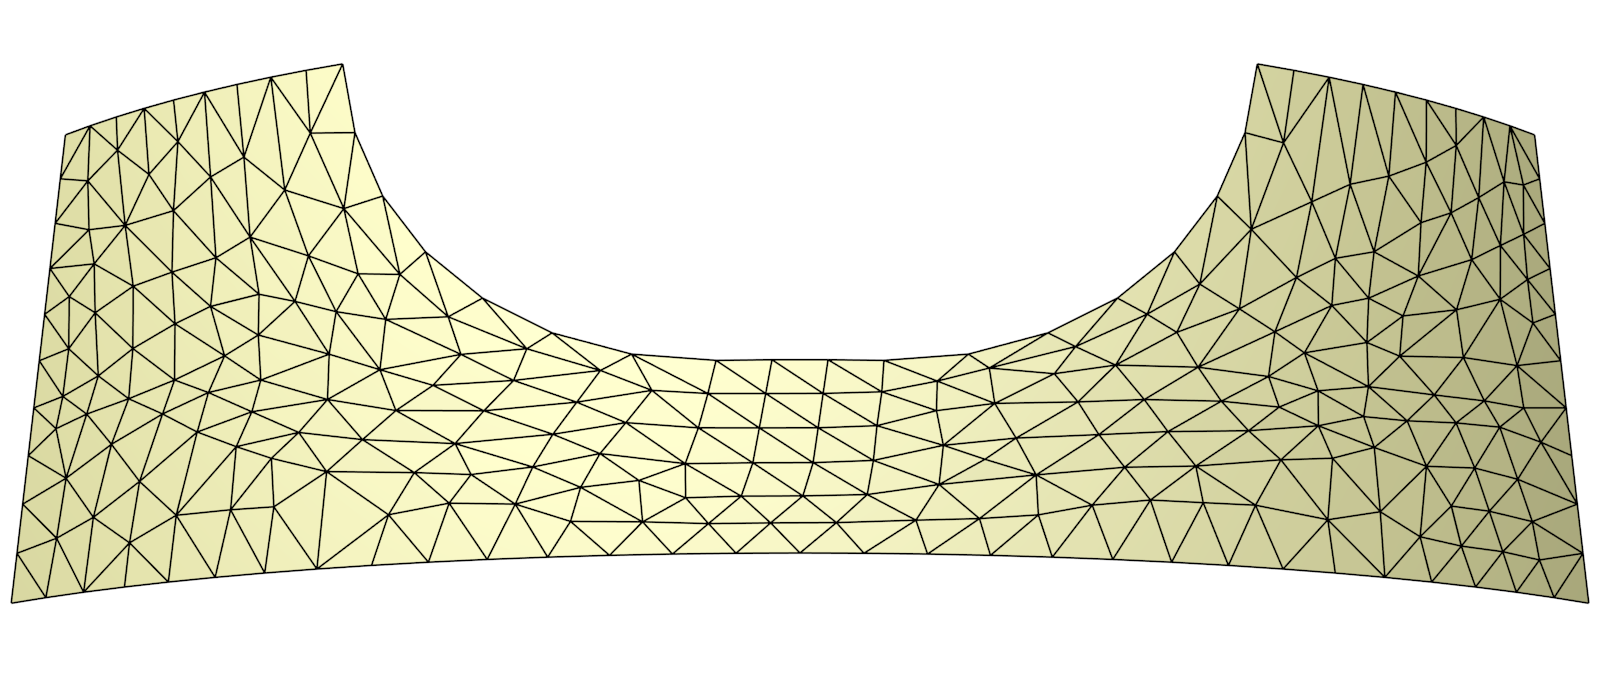
\includegraphics[height=20mm]{mesh_1c}
	\begin{tikzpicture}
		\begin{semilogyaxis}[%
			width=0.95\linewidth, height=0.8\linewidth,%
			xmin=0.0, xmax=70.0, ymin=1.0e-16, ymax=1.0e1,%
			grid=major,%
			xlabel={$n$},%
			ylabel={$\left | \hat{f}_n \right |$},%
			xtick distance=10,%
			ytick={1e-15,1e-10,1e-5,1e0},%
			legend pos=south west,%
			legend style={font=\small},%
			samples=100,%
%			mark options={scale=.8}%
		]%
		\addplot+[only marks] table[x expr=\coordindex, y index=0] {figures/data/coeffs.dat}; 
		\addplot+[only marks] table[x expr=\coordindex, y index=1] {figures/data/coeffs.dat}; 
		\addplot+[only marks] table[x expr=\coordindex, y index=2] {figures/data/coeffs.dat}; 
%		\addplot+[dashed, color=black, no marks, very thick][domain=5.0:60.0] {2.0*exp(-0.5*x)};
		\addplot+[dashed, color=black, no marks, very thick][domain=30.5:59.5] {1e6*exp(-0.5*x)};
		\legend{{$f$},{$f'$},{$f''$},{$e^{-0.5n}$}}
%		\legend{
%		{$\left | \tilde{f}_n \right |$},
%		{$\left | \tilde{f}^{(1)}_n \right |$},
%		{$\left | \tilde{f}^{(2)}_n \right |$},
%		{$e^{-0.5n}$}}
		\end{semilogyaxis}%
	\end{tikzpicture}
  }\hfill\null
  \vspace{\onelineskip}%\hrule
  \null\hfill\parbox[t]{0.48\linewidth}{%
  	\caption{Error in approximating the analytic function $f : x \mapsto e^{\sin 3 x^3}$ and its first two derivatives by their truncated Chebyshev series. The black, dotted curve shows the exponential rate of convergence.}\label{fig:convergence_interpolant}%
  }\hfill
  \parbox[t]{0.48\linewidth}{%
    \caption{Exponential decay of the Chebyshev coefficients of the analytic function $f : x \mapsto e^{\sin 3 x^3}$ and its first two derivatives.}%
  	\label{fig:convergence_coeffs}%
  }\hfill\null
\end{figure}

\lipsum[8-9]



\begin{figure}
  \centering
  \begin{minipage}{0.4\textwidth}
    \centering
    %GRAPHIC 1
    
\includegraphics[height=45mm]{imr_trimmed_patch_xyz}
    \caption{Graphic 1 in a float} \label{fig:mult2}
  \end{minipage}
  \hfill
  \begin{minipage}{0.4\textwidth}
    \centering
    %GRAPHIC 2
    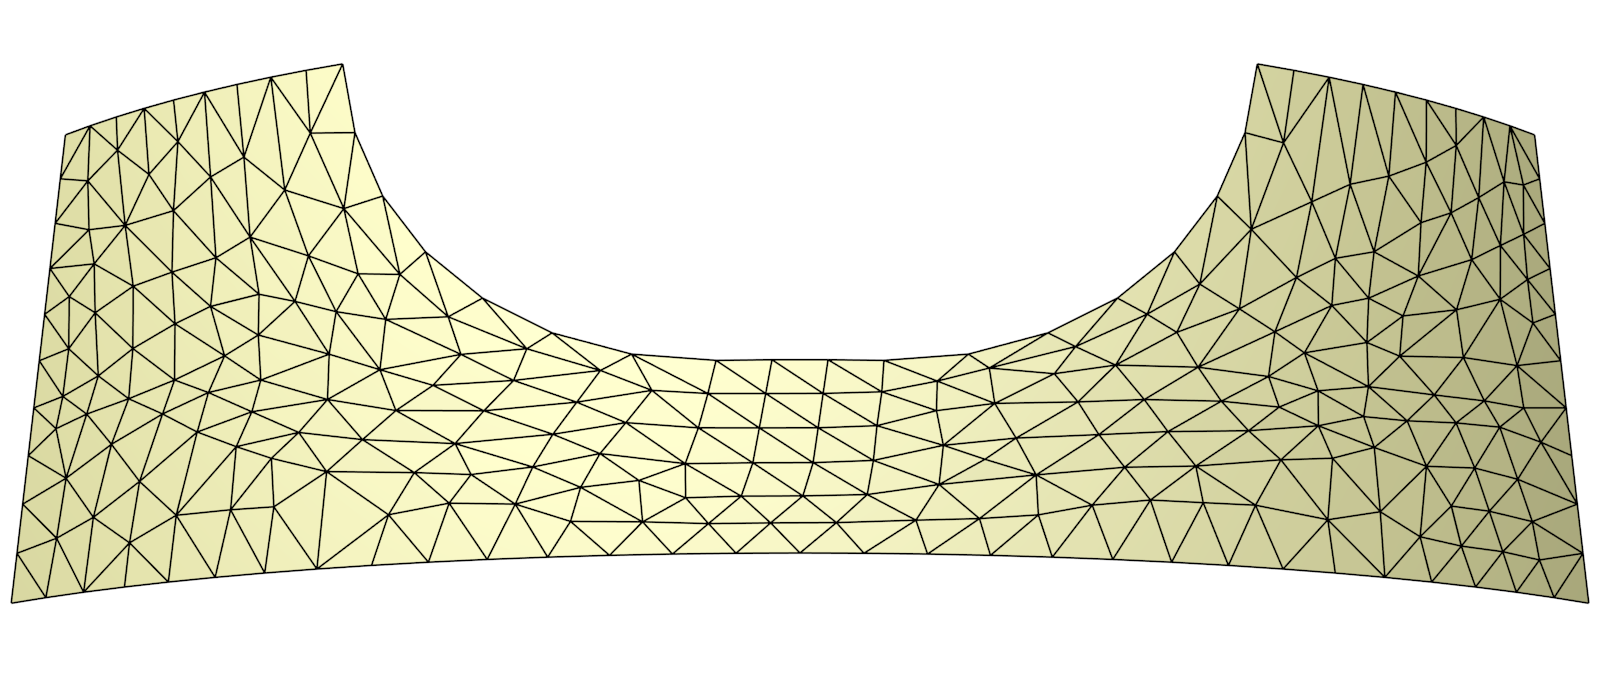
\includegraphics[height=20mm]{mesh_1c}
    \caption{Graphic 2 in same float} \label{fig:mult3}
  \end{minipage}
\end{figure}

\lipsum[8-15]

\begin{figure}
  \vspace{\onelineskip}
  \null\hfill\parbox{0.48\linewidth}{%
    \centering
    %Aligned to the center of the right figure
    
\includegraphics[height=45mm]{imr_trimmed_patch_xyz}
  }\hfill
  \parbox{0.48\linewidth}{%
    \centering
%     This is the right figure which is taller
%     than the first one (the one at the left)
	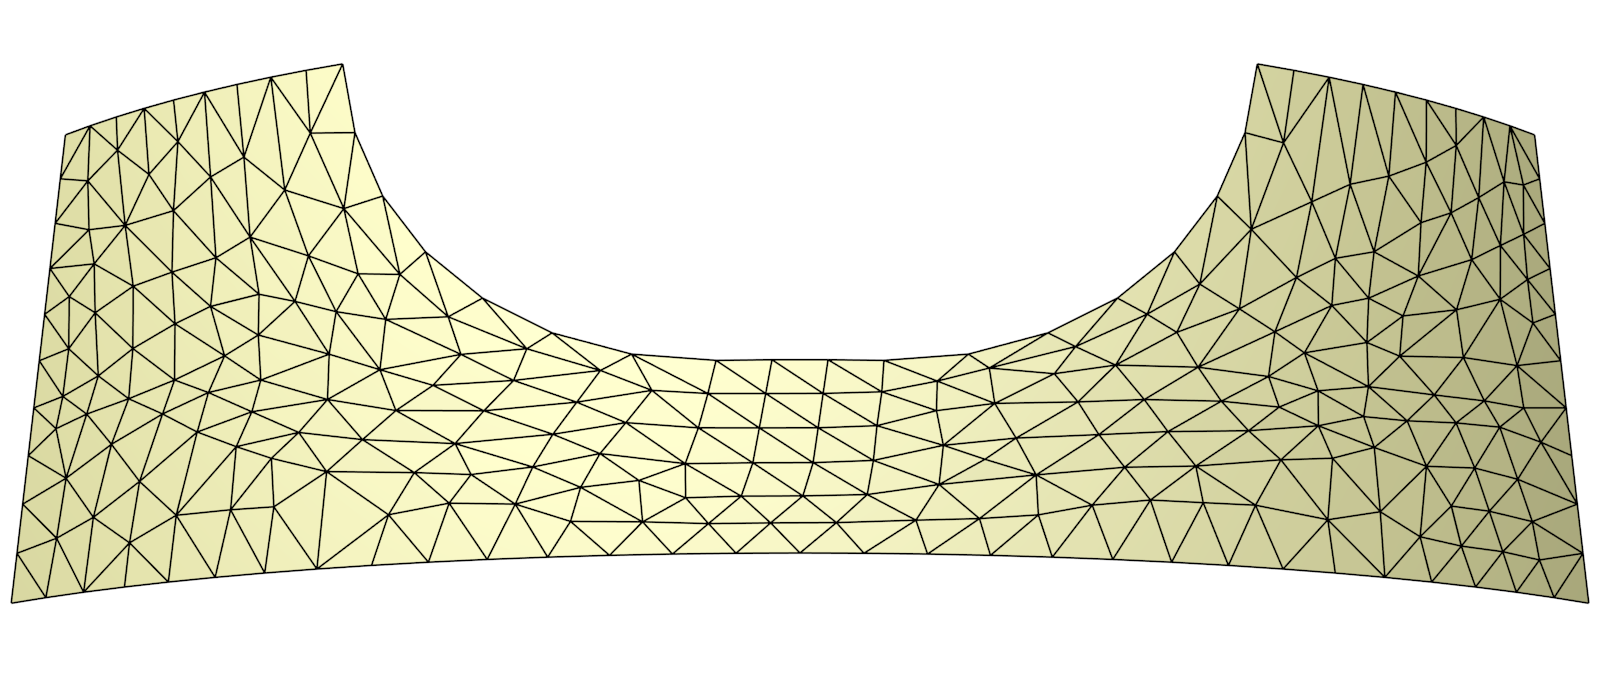
\includegraphics[height=20mm]{mesh_1c}
  }\hfill\null
  \vspace{\onelineskip}%\hrule
  \null\hfill\parbox[t]{0.48\linewidth}{%
  	\caption{Left figure}\label{fig:left1}%
  }\hfill
  \parbox[t]{0.48\linewidth}{%
    \caption{Right figure. This has more text than the adjacent
    caption (\ref{fig:left1}) so the heights are unequal}%
  	\label{fig:right1}%
  }\hfill\null
\end{figure}




\begin{figure}
  \centering
  \hspace*{\fill}
  \subbottom[Subfigure 1]{
  
\includegraphics[height=45mm]{imr_trimmed_patch_xyz}
  %\fbox{SUBFIGURE ONE}\label{sf:1}
  }
  \hfill
  \subbottom[Subfigure 2]{
  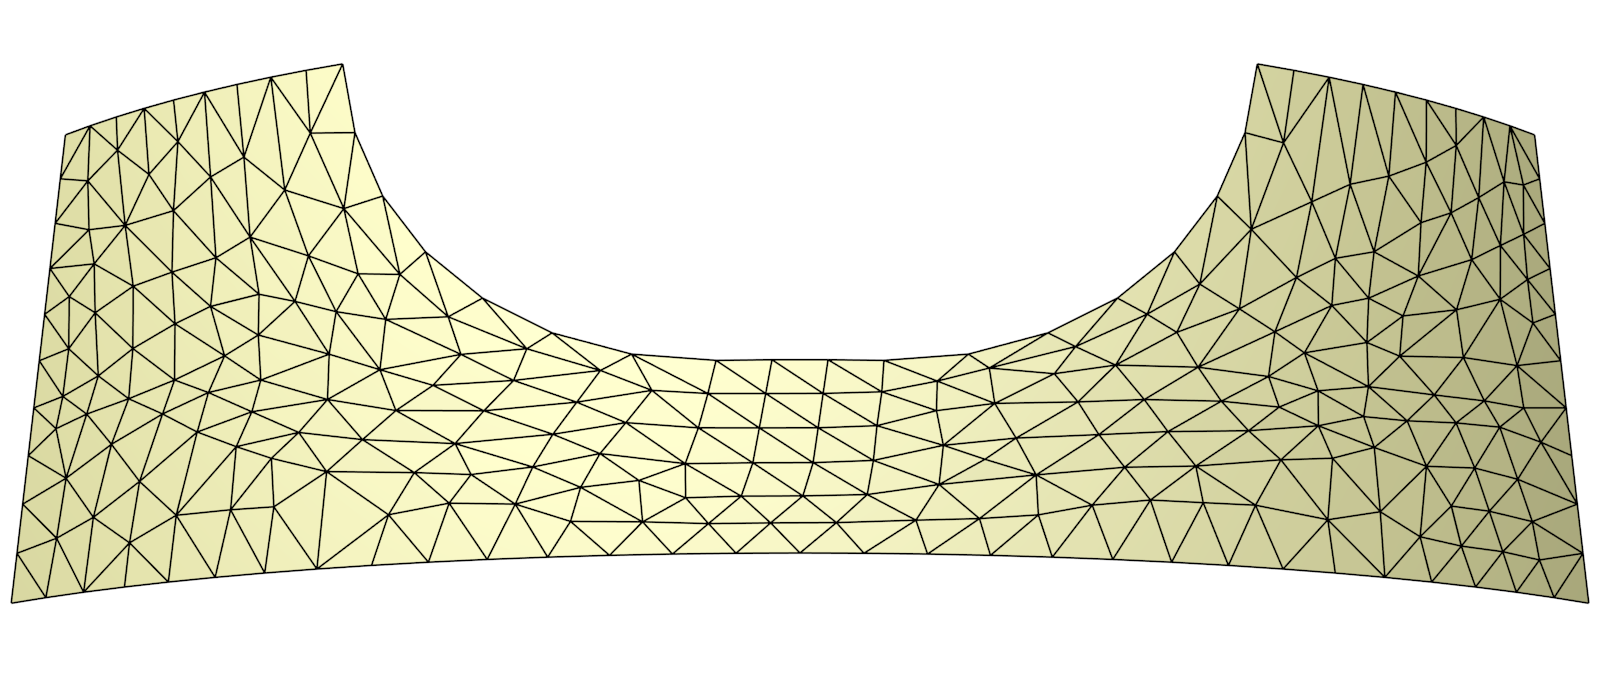
\includegraphics[height=20mm]{mesh_1c}
  %\fbox{SUBFIGURE TWO}\label{sf:2}
  }
  \hspace*{\fill}
  \caption{Figure with two subfigures} \label{fig:twosubfig}
\end{figure}


% \begin{figure}
%   \centering
%   \begin{minipage}{0.3\textwidth}
%     Some verbatim text
%     \subcaption{First text}
%   \end{minipage}
%   \hfill
%   \begin{minipage}{0.3\textwidth}
%     More verbatim text
%     \subcaption{Second text}
%   \end{minipage}
%   \caption{Verbatim texts}
% \end{figure}


\begin{figure}
  \centering
  \hspace*{\fill}
  \subbottom[Subfigure 1]{
  
\includegraphics[height=45mm]{imr_trimmed_patch_xyz}
  %\fbox{SUBFIGURE ONE}\label{sf:1}
  }
  \hfill
  \begin{tikzpicture}
      \useasboundingbox (0,0) rectangle(3cm,5cm);
	  \coordinate (a) at (5mm,45mm);
	  \draw[-latex] (a) to ([yshift=-3cm]a) node [left] {$x$};
	  \draw[-latex] (a) to node [above] {$y$} ([xshift=2cm]a);
  \end{tikzpicture}
  \hfill
  \subbottom[Subfigure 2]{
  
\includegraphics[height=45mm]{imr_trimmed_patch_xyz}
  %\fbox{SUBFIGURE TWO}\label{sf:2}
  }
  \hspace*{\fill}
  \caption{Figure with two subfigures} 
\end{figure}
